\section{Visualización de la simulación}

Para verificar visualmente el resultado usé el script provisto por la cátedra (show\_blue2red.py), que lee los frames binarios que el programa guarda en cada paso y los anima como un mapa de calor, de azul (0°C) a rojo (100°C). Las capturas corresponden a una simulación lanzada con los siguientes parámetros: N = 256, 200 pasos y 256 hilos por bloque.

\begin{figure}[H]
    \centering
    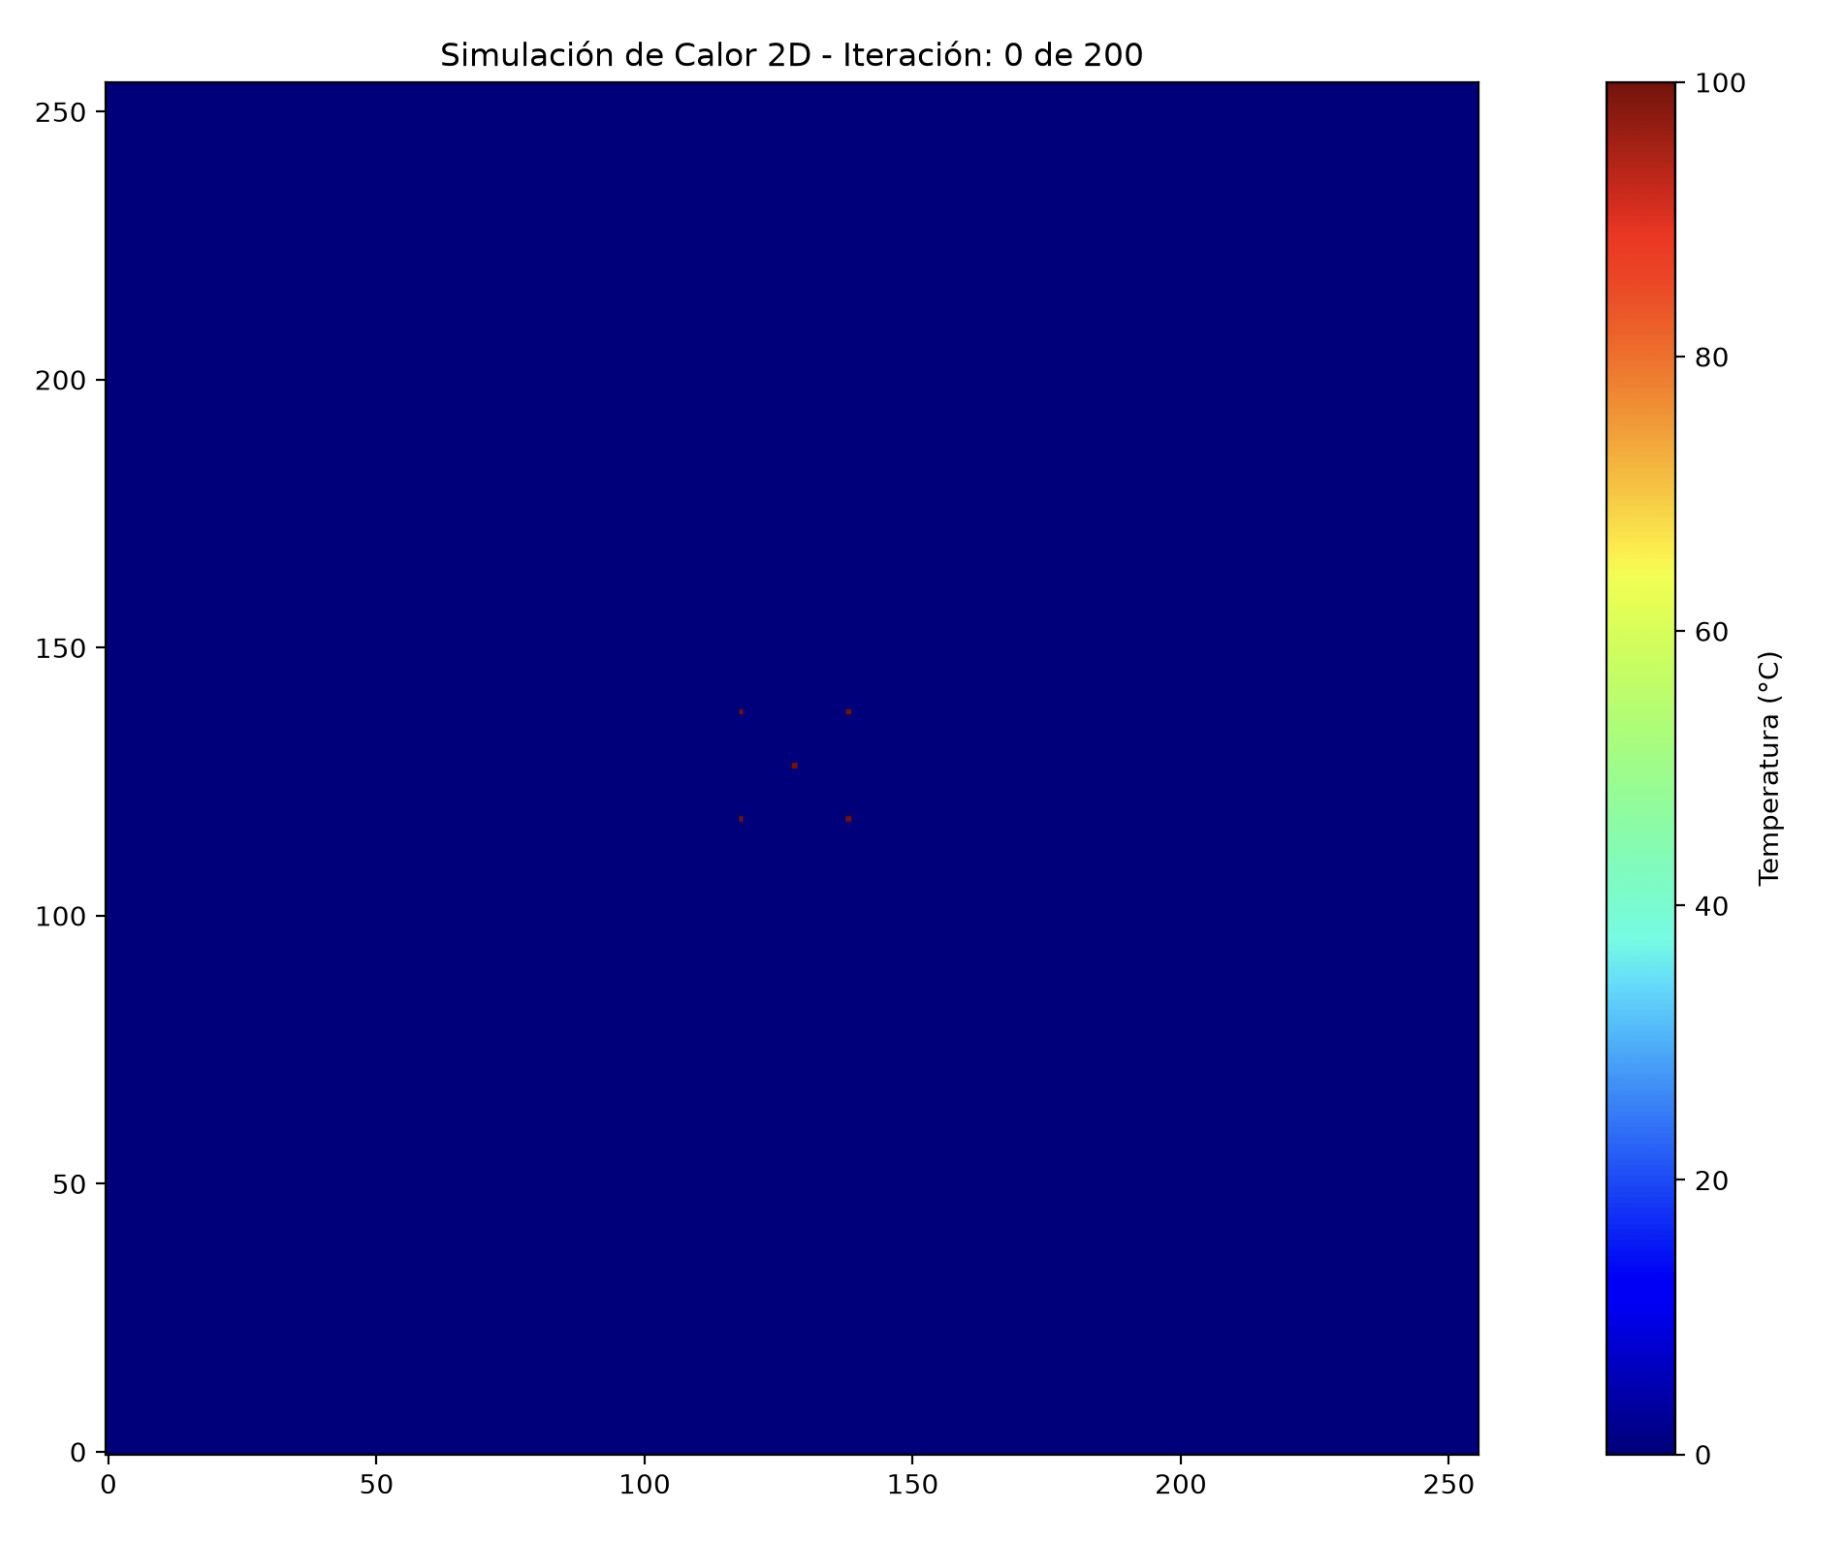
\includegraphics[width=1\textwidth]{secciones/imagenes/it0_gpu.png}
    \caption{Estado inicial con las 5 fuentes de calor centrales en 100 grados}
    \label{fig:paso0}
\end{figure}

\begin{figure}[H]
    \centering
    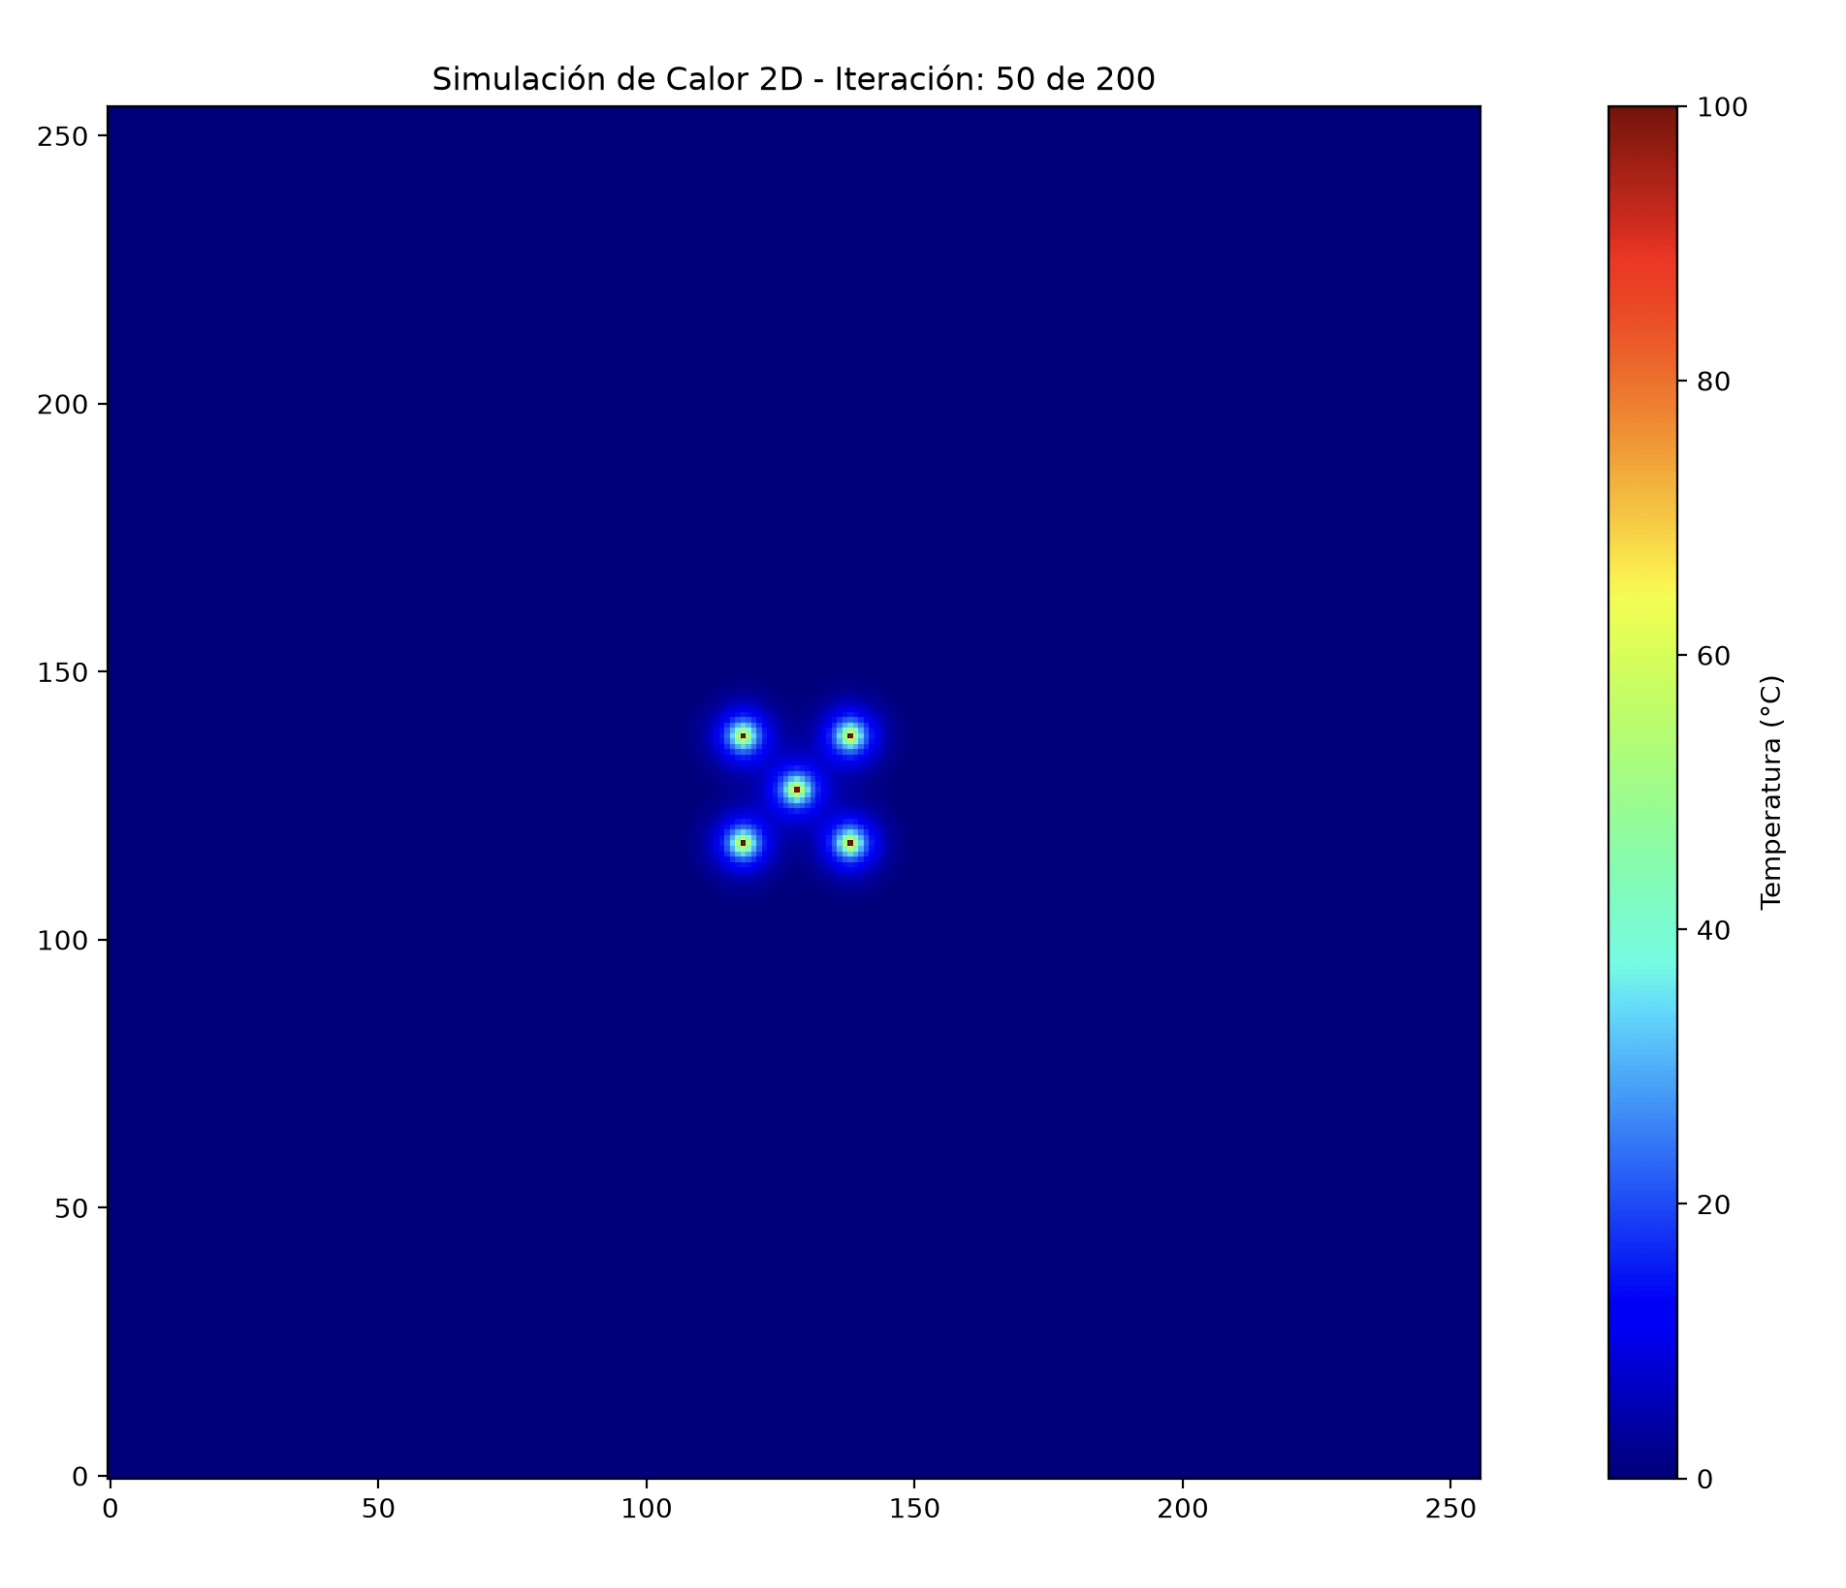
\includegraphics[width=0.65\textwidth]{secciones/imagenes/it50_gpu.png}
    \caption{Paso 50}
    \label{fig:paso50}
\end{figure}

\begin{figure}[H]
    \centering
    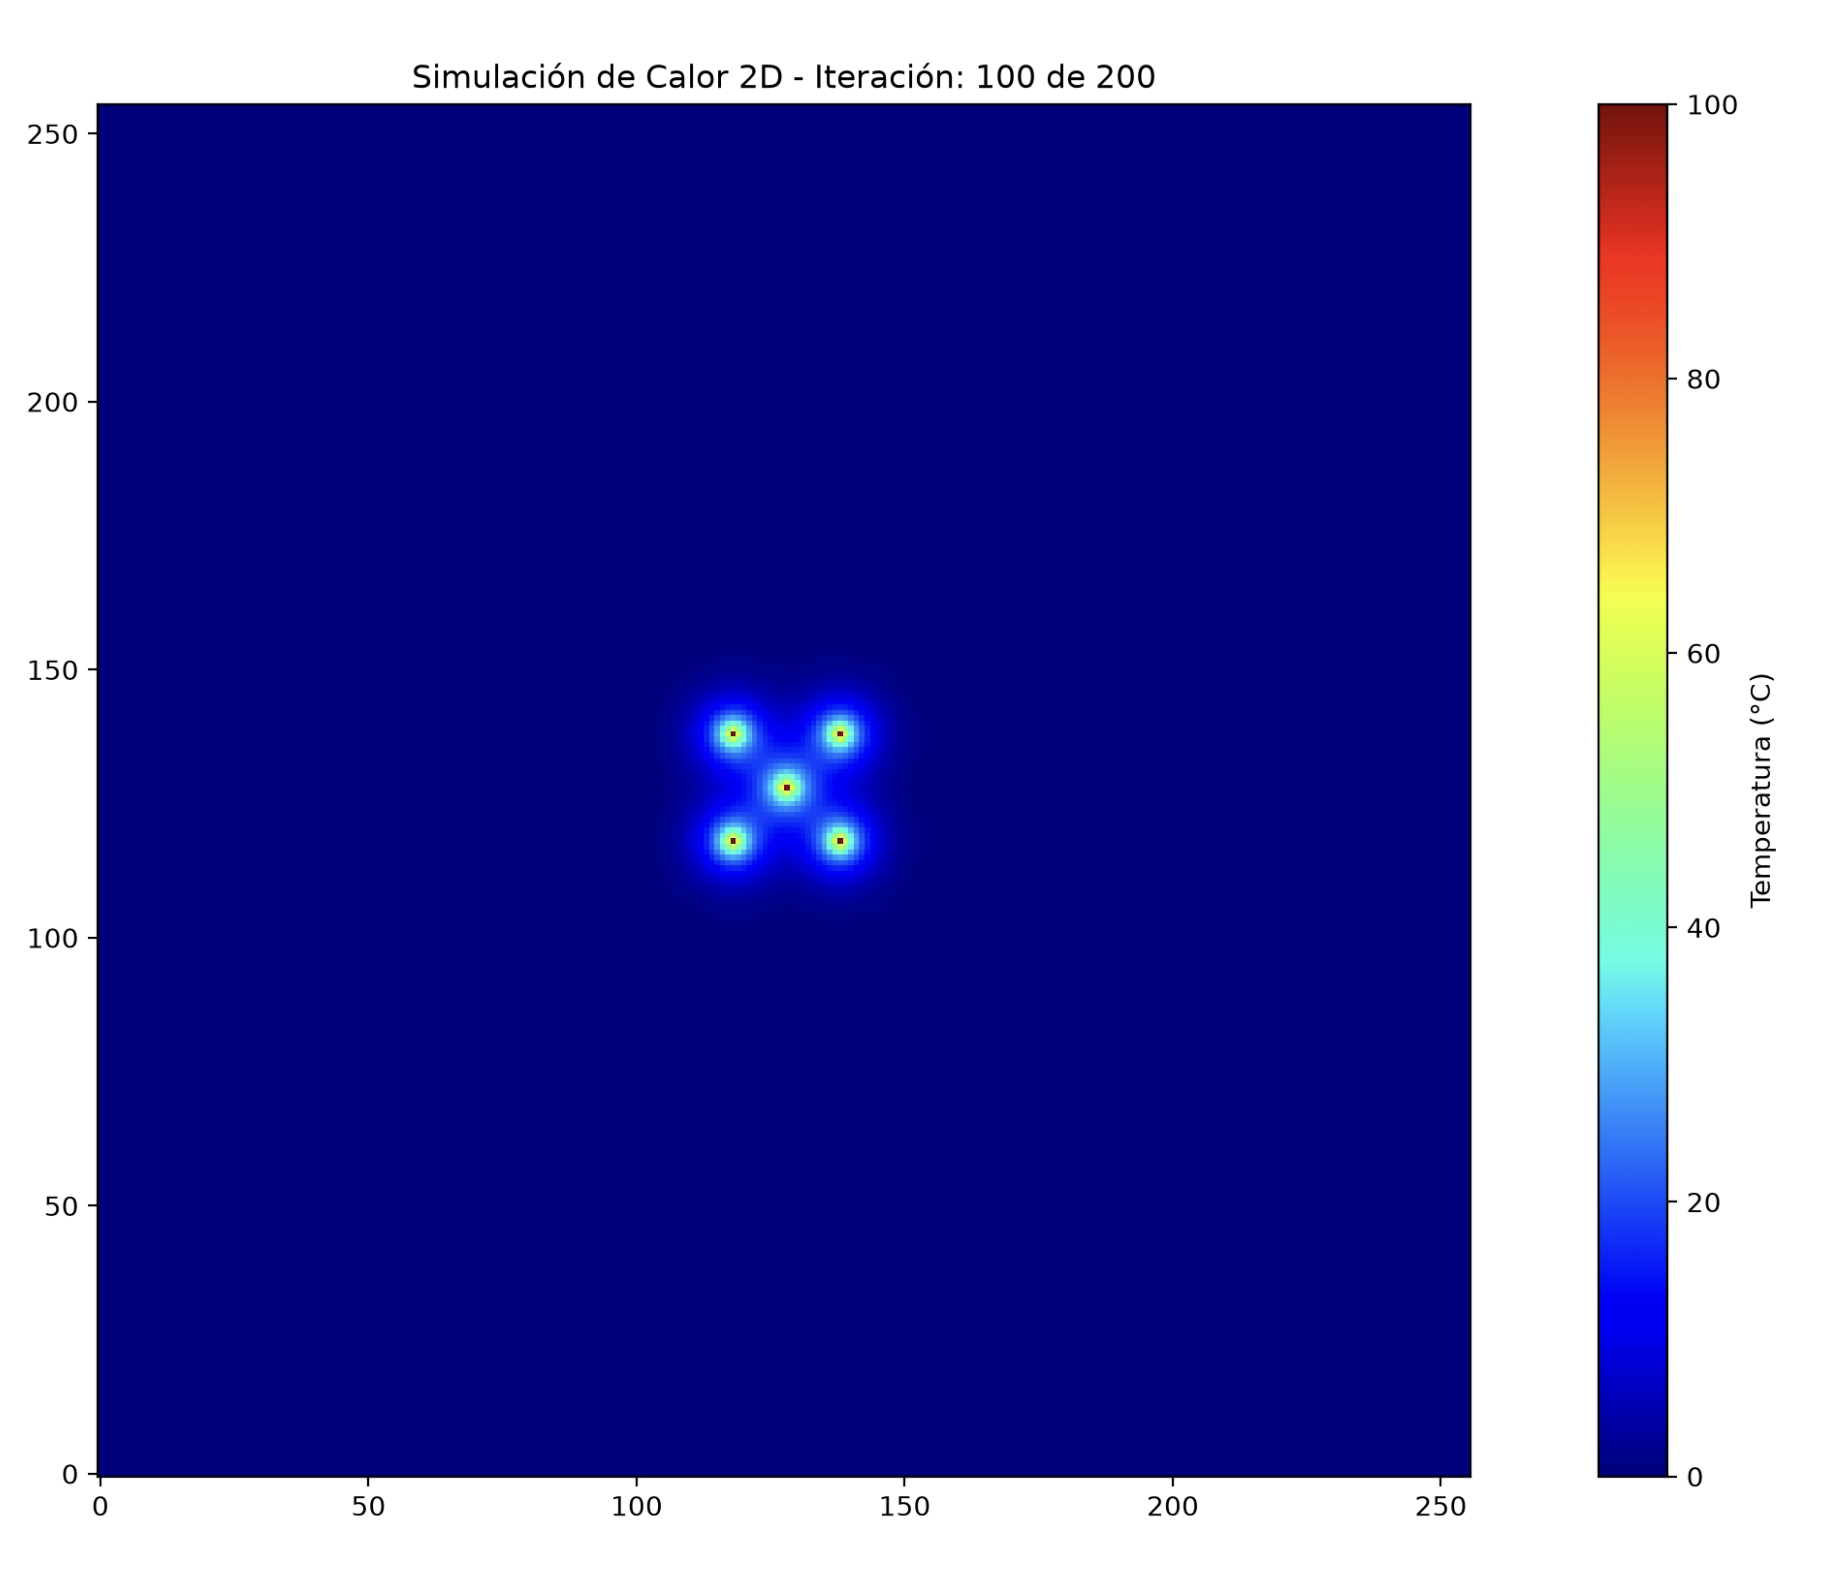
\includegraphics[width=0.65\textwidth]{secciones/imagenes/it100_gpu.png}
    \caption{Paso 100}
    \label{fig:paso100}
\end{figure}

\begin{figure}[H]
    \centering
    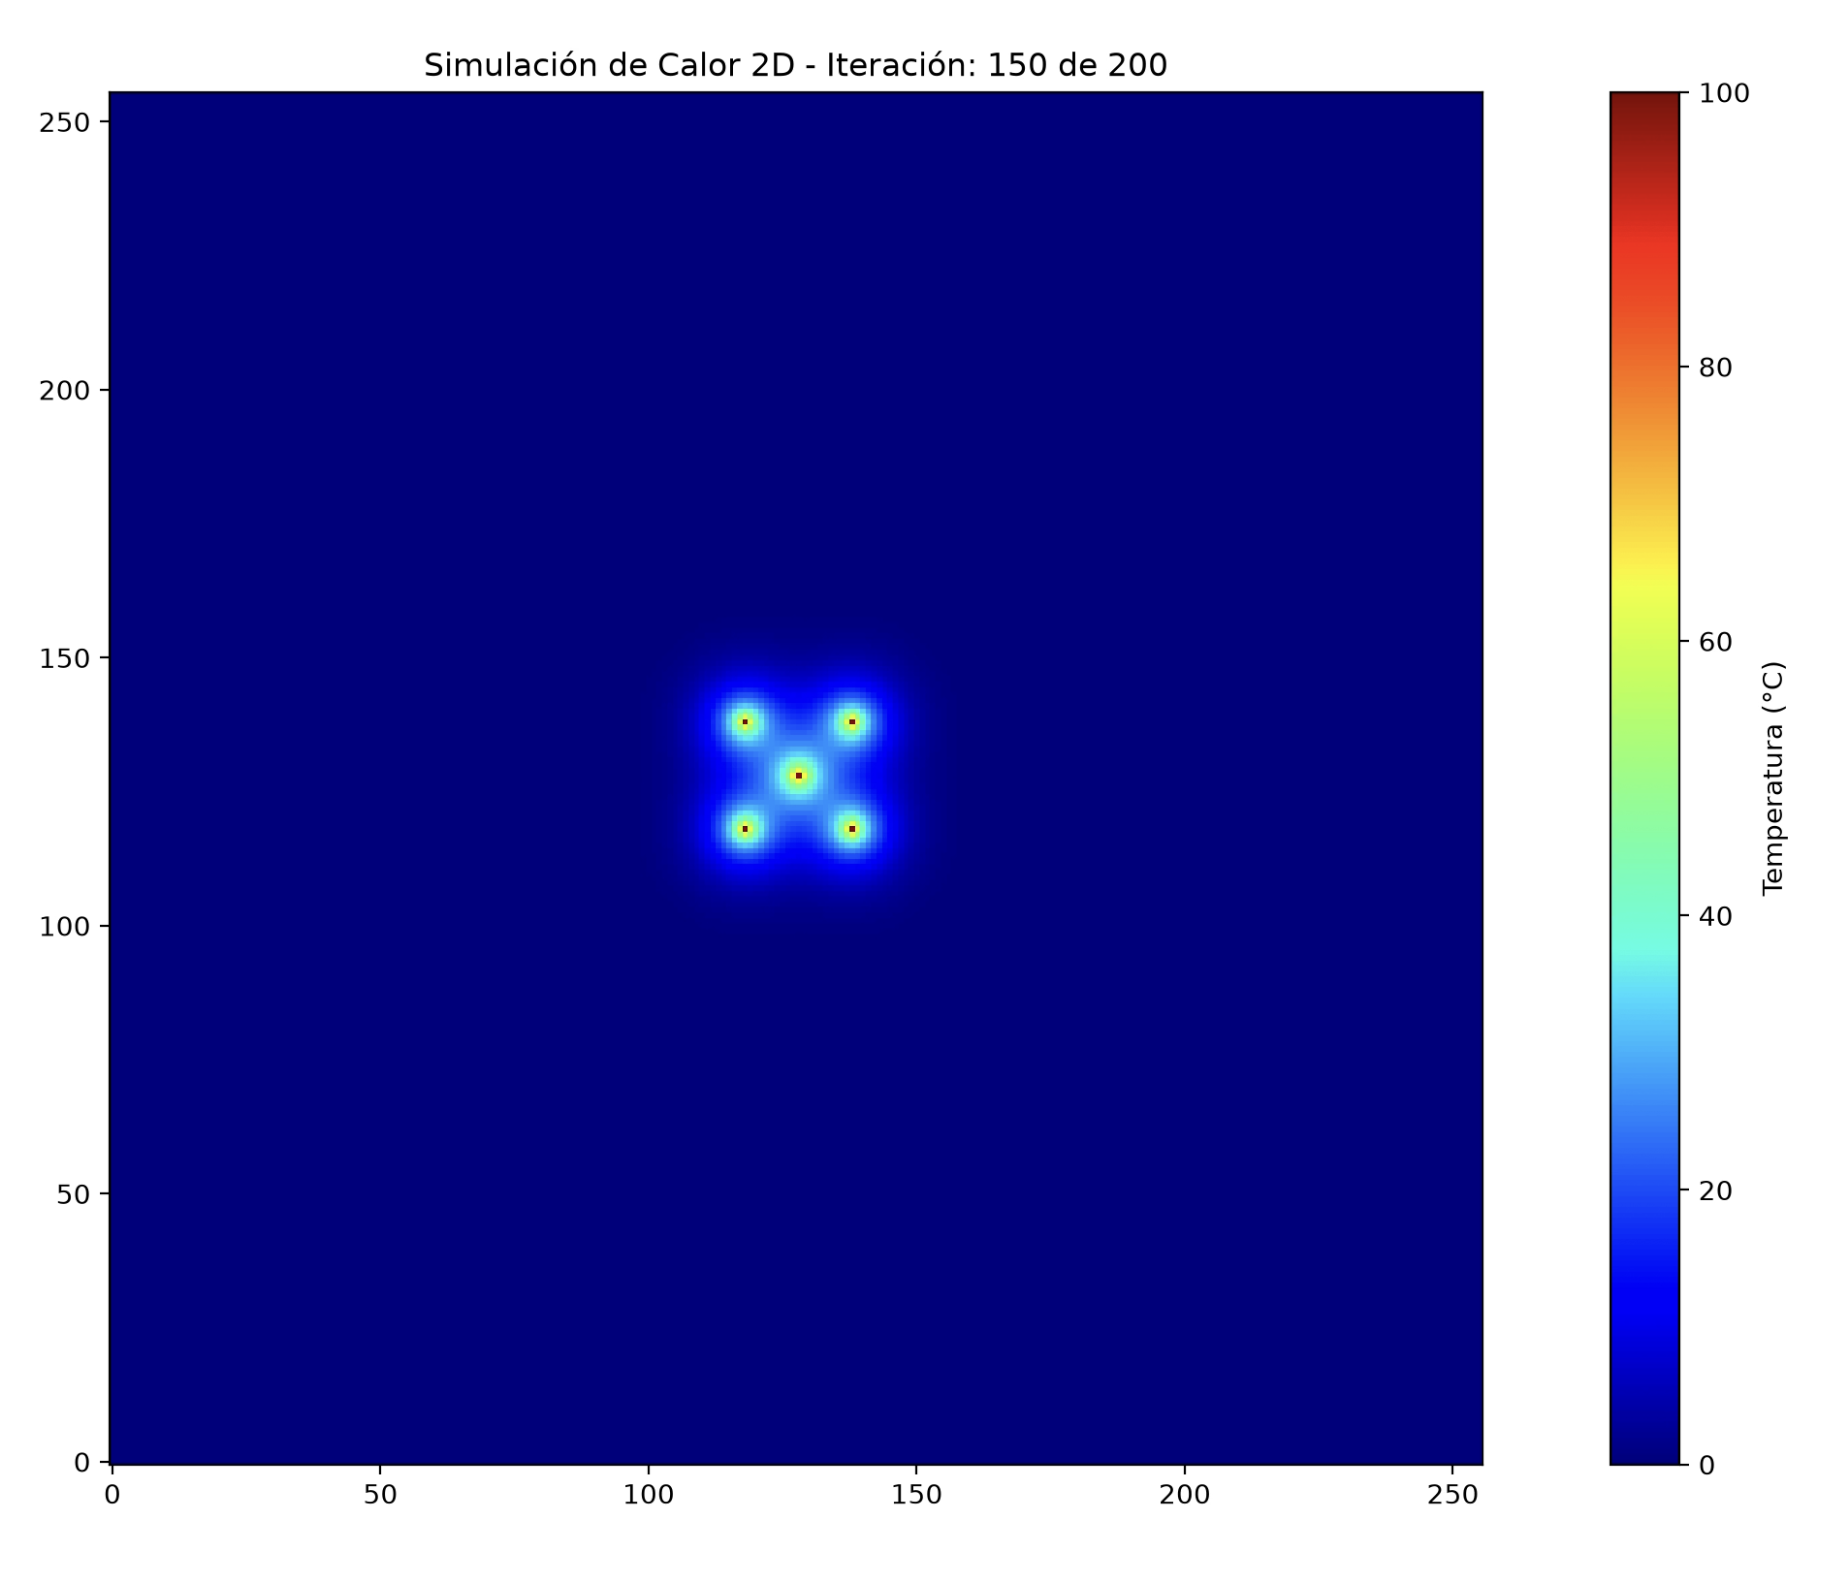
\includegraphics[width=0.65\textwidth]{secciones/imagenes/it150_gpu.png}
    \caption{Paso 150}
    \label{fig:paso150}
\end{figure}

\begin{figure}[H]
    \centering
    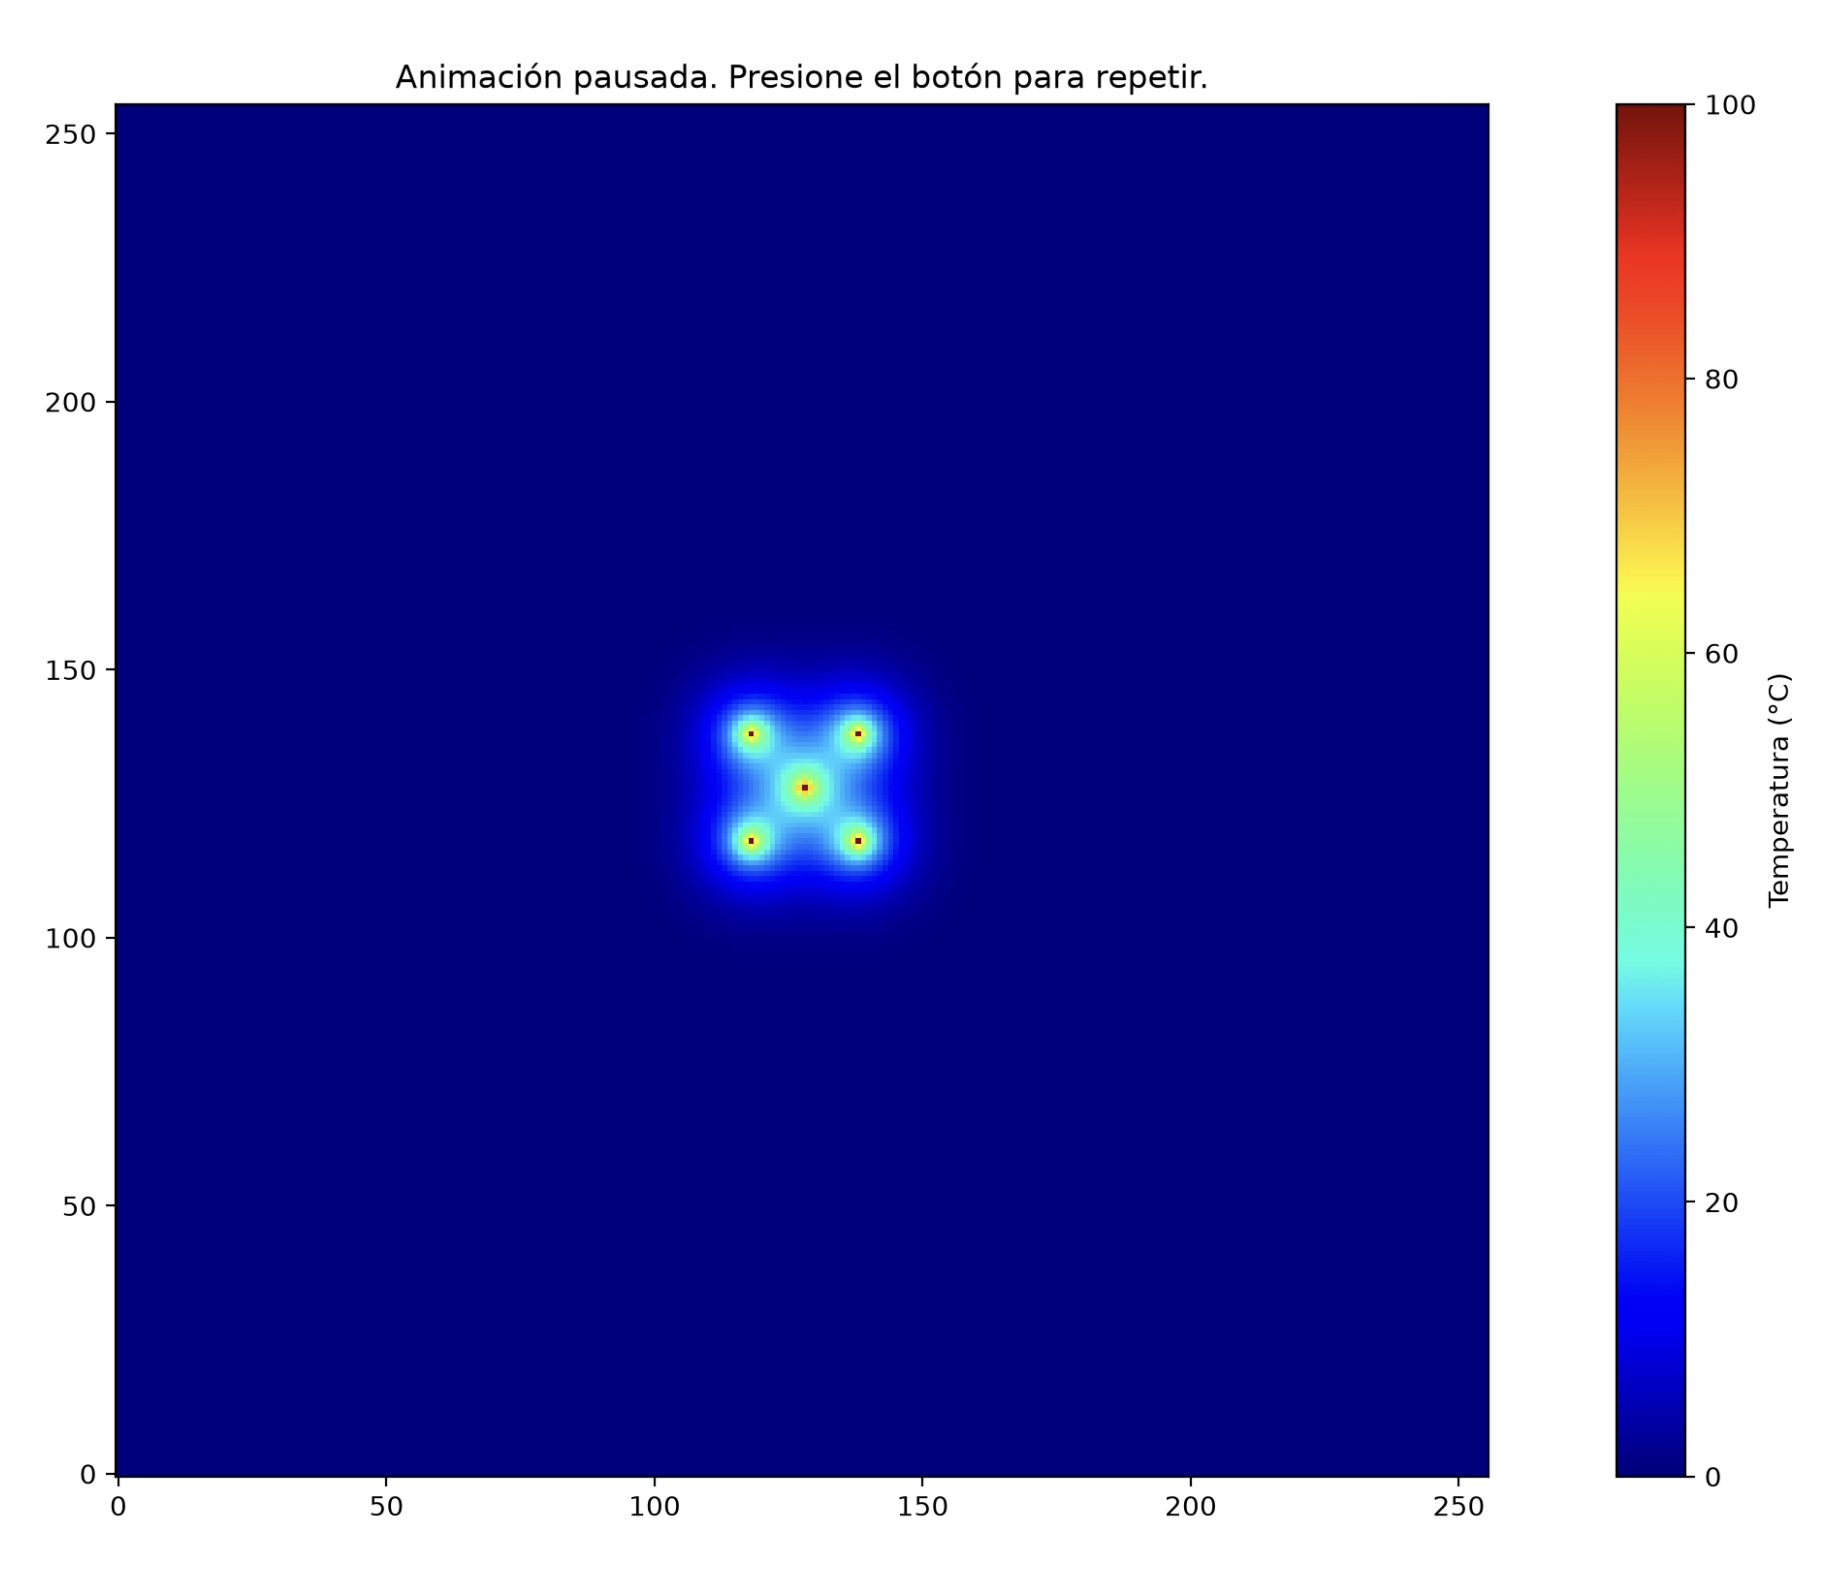
\includegraphics[width=0.65\textwidth]{secciones/imagenes/it200_gpu.png}
    \caption{Estado final de la simulación (paso 200)}
    \label{fig:paso200}
\end{figure}